\documentclass{standalone}

\usepackage{tikz}
\usetikzlibrary{calc, intersections}


\begin{document}
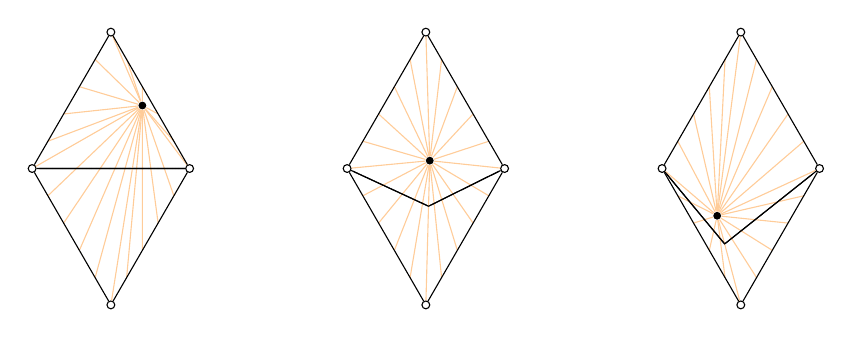
\begin{tikzpicture}[scale=2]
  \pgfmathsetmacro{\y}{sqrt(3)/2}
  \pgfmathsetmacro{\xl}{1/2}

  \def\drawss{
    % Name the vertices of the simplex
    % a
    % / \
    % c - b
    % \ /
    % d
    %
    \node[circle, draw=black, fill=white, inner sep=1pt] (a) at (0,\y) {};
    \node[circle, draw=black, fill=white, inner sep=1pt] (b) at (\xl,0) {};
    \node[circle, draw=black, fill=white, inner sep=1pt] (c) at (-\xl,0) {};
    \node[circle, draw=black, fill=white, inner sep=1pt] (d) at (0,-\y) {};

    \foreach \rat in {1,2,...,4}{
      \pgfmathsetmacro{\ratfrac}{\rat/5}
      \pgfmathsetmacro{\compratf}{1 - \ratfrac}

      \coordinate (ab\rat) at ($\ratfrac*(a) + \compratf*(b)$);
      \coordinate (ac\rat) at ($\ratfrac*(a) + \compratf*(c)$);
      \coordinate (bd\rat) at ($\ratfrac*(b) + \compratf*(d)$);
      \coordinate (cd\rat) at ($\ratfrac*(c) + \compratf*(d)$);
      \draw[orange!40!white] (ab\rat) -- (dpoint) (ac\rat) --
      (dpoint) (bd\rat) -- (dpoint) (cd\rat) -- (dpoint);
    }

    % Draw the lines from the vertices to the moving point
    \draw[orange!40!white] (a) -- (dpoint) (b) -- (dpoint) (c) -- (dpoint) (d) -- (dpoint);

    % OK, now to draw the middle line.
    %
    % The middle line gets a special name since we're gonna
    % use the intersections to deform it
    \path[name path=middle] (b) -- (c);

    % Approximate by 30 line segments
    \pgfmathsetmacro{\numsamps}{40}
    \foreach \rat in {1,2,...,\numsamps}{
      \pgfmathsetmacro{\ratfrac}{\rat/(\numsamps+1)}
      \pgfmathsetmacro{\compratf}{1 - \ratfrac}

      % We'll assume the point starts in the upper-right area,
      % so we only need to look at lines coming from points
      % connected to (d)
      \coordinate (bd\rat) at ($\ratfrac*(b) + \compratf*(d)$);
      \coordinate (cd\rat) at ($\ratfrac*(c) + \compratf*(d)$);

      \path[name path=pbd] (bd\rat) -- (sspoint);
      \path[name path=pcd] (cd\rat) -- (sspoint);

      \path[name intersections={of=pbd and middle, by=bdi}];
      \path[name intersections={of=pcd and middle, by=cdi}];

      % Ok: the intersection points are of the form t*end +
      % (1-t)*start, where end is a point on the line segment
      % bd, and start is the original start point (sspoint).
      %
      % We need to solve for t. Here, end is
      % (sspoint), and start is (bd\rat) or (cd\rat).
      %
      % We'll write it out for bdi.
      %
      % t*end + (1-t) * start = bdi
      % t*(end - start) + start = bdi
      % bdi - start = t*(end - start)
      % So (bdi-start)[0]/(end - start)[0] = t.
      %
      % Let's do it. We define the difference vectors
      \coordinate (bdidiff) at ($(bdi) - (sspoint)$);
      \coordinate (ebdiff) at ($(bd\rat) - (sspoint)$);

      \coordinate (cdidiff) at ($(cdi) - (sspoint)$);
      \coordinate (ecdiff) at ($(cd\rat) - (sspoint)$);


      \path let \p1 = (bdidiff), \p2 = (ebdiff) in coordinate
      (bmid\rat) at ($\x1/\x2*(bd\rat) - \x1/\x2*(dpoint)$);
      \coordinate (bmid\rat) at ($(bmid\rat) + (dpoint)$);

      % \coordinate (idk1) at ($(idk1)+.5*(b)$);

      \path let \p1 = (cdidiff), \p2 = (ecdiff) in coordinate
      (cmid\rat) at ($\x1/\x2*(cd\rat) - \x1/\x2*(dpoint)$);
      \coordinate (cmid\rat) at ($(cmid\rat) + (dpoint)$);

      % \node[circle, fill=red, inner sep=.2pt] at (idk1) {};
      % \node[circle, fill=blue, inner sep=.2pt] at (idk2) {};
      % \node[circle, fill=red, inner sep=.1pt] at (bdidiff) {};
      % \node[circle, fill=blue, inner sep=.1pt] at (ebdiff) {};
      % \node[circle, fill=white, inner sep=1pt] at (sspoint) {};
      % \node[circle, fill=red, inner sep=.1pt] at (bdidiff) {};

      % \node[circle, fill=green, inner sep=1pt] at (epoint) {};
      % \node[circle, fill=black, inner sep=.1pt] at (bdi) {};
      % \coordinate (bdix) at ($(bdidiff)!(0,0)!(1,0)$);
      % \coordinate (essx) at ($(essdiff)!(0,0)!(1,0)$);
    }

    % Finally, we do it for d as well
    \path[name path=pdd] (d) -- (sspoint);
    \path[name intersections={of=pdd and middle, by=ddi}];
    \coordinate (ddidiff) at ($(ddi) - (sspoint)$);
    \coordinate (eddiff) at ($(d) - (sspoint)$);

    \path let \p1 = (ddidiff), \p2 = (eddiff) in coordinate
    (dmid) at ($\x1/\x2*(d) - \x1/\x2*(dpoint)$);
    \coordinate (dmid) at ($(dmid) + (dpoint)$);


    \draw (c)--(cmid1) (cmid\numsamps) -- (dmid) --
    (bmid\numsamps) (b)--(bmid1);

    % Draw boundary of simplex
    \draw (a) -- (b) -- (d) -- (c) -- (a);

    \foreach \rat in {2,3,...,\numsamps}{
      \pgfmathsetmacro{\prevrat}{\rat-1}
      \draw[] (cmid\prevrat) -- (cmid\rat);
      \draw[] (bmid\prevrat) -- (bmid\rat);

    }
  }

  % Start point and endpoint
  \coordinate (spoint) at (.2, .4);
  \coordinate (epoint) at (-.15, -.3);

  \begin{scope}[xshift=-2cm]
    \coordinate (sspoint) at ($(spoint) + (-2.,0.)$);
    \node[circle, fill=black, inner sep=1pt] (dpoint) at (.2,
    .4) {};
    \drawss
  \end{scope}

  \begin{scope}[xshift=0cm]
    \coordinate (sspoint) at (spoint);
    \node[circle, fill=black, inner sep=1pt] (dpoint) at
    ($.5*(spoint) + .5*(epoint)$) {};
    \drawss
  \end{scope}

  \begin{scope}[xshift=2cm]
    \coordinate (sspoint) at ($(spoint) + (2.,0.)$);
    \coordinate (epoint) at (-.15, -.3);
    \node[circle, fill=black, inner sep=1pt] (dpoint) at
    (epoint) {};
    \drawss
  \end{scope}
\end{tikzpicture}
\end{document}
